\hypertarget{pf__search_8h}{
\section{pf\_\-search.h File Reference}
\label{pf__search_8h}\index{pf\_\-search.h@{pf\_\-search.h}}
}


This graph shows which files directly or indirectly include this file:\nopagebreak
\begin{figure}[H]
\begin{center}
\leavevmode
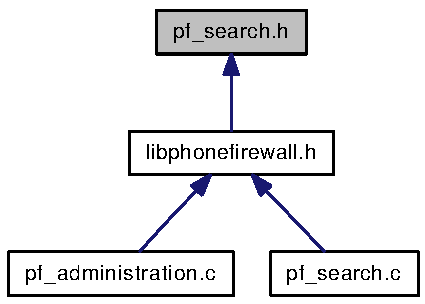
\includegraphics[width=120pt]{pf__search_8h__dep__incl}
\end{center}
\end{figure}
\subsection*{Functions}
\begin{CompactItemize}
\item 
struct \hyperlink{structEntry}{Entry} $\ast$ \hyperlink{pf__search_8h_3947a1543660e9f6e666242efee44f89}{get\_\-entry\_\-by\_\-name} (char $\ast$name, int listflag)
\item 
struct \hyperlink{structEntry}{Entry} $\ast$ \hyperlink{pf__search_8h_678d356be18c20e298d74a62bc6e8782}{get\_\-entry\_\-by\_\-number} (int country\_\-code, int area\_\-code, unsigned long long number, int listflag)
\item 
struct \hyperlink{structEntry}{Entry} $\ast$ \hyperlink{pf__search_8h_b4e0af5dc1b0cf0bdd5812c973dcd353}{get\_\-entry\_\-by\_\-reason} (char $\ast$reason, int listflag)
\end{CompactItemize}


\subsection{Function Documentation}
\hypertarget{pf__search_8h_3947a1543660e9f6e666242efee44f89}{
\index{pf\_\-search.h@{pf\_\-search.h}!get\_\-entry\_\-by\_\-name@{get\_\-entry\_\-by\_\-name}}
\index{get\_\-entry\_\-by\_\-name@{get\_\-entry\_\-by\_\-name}!pf_search.h@{pf\_\-search.h}}
\subsubsection{\setlength{\rightskip}{0pt plus 5cm}struct {\bf Entry}$\ast$ get\_\-entry\_\-by\_\-name (char $\ast$ {\em name}, int {\em listflag})\hspace{0.3cm}{\tt  \mbox{[}read\mbox{]}}}}
\label{pf__search_8h_3947a1543660e9f6e666242efee44f89}


Search a \hyperlink{structentry}{entry} by name.

\begin{Desc}
\item[Parameters:]
\begin{description}
\item[{\em name}]The name of the person which is blocked. \item[{\em listflag}]A flag, which indicates if you would use the blacklist (BLACKLIST\_\-FLAG) or the whitelist (WHITELIST\_\-FLAG).\par
\end{description}
\end{Desc}
\begin{Desc}
\item[Returns:]\hyperlink{structentry}{entry} Returns the entries which are found in a linked list. \end{Desc}


Definition at line 112 of file pf\_\-search.c.

References ASCII\_\-PERCENT\_\-CHAR, DB\_\-FILE, ERR\_\-LOG, find\_\-entry(), insert\_\-into\_\-list(), MAX\_\-LINE\_\-LENGTH, STMT\_\-SIZE, TB\_\-AREACODE, TB\_\-COUNTRYCODE, TB\_\-NAME, TB\_\-NUMBER, TB\_\-PRIORITY, TB\_\-REASON, and WHITELIST\_\-FLAG.

Here is the call graph for this function:\nopagebreak
\begin{figure}[H]
\begin{center}
\leavevmode
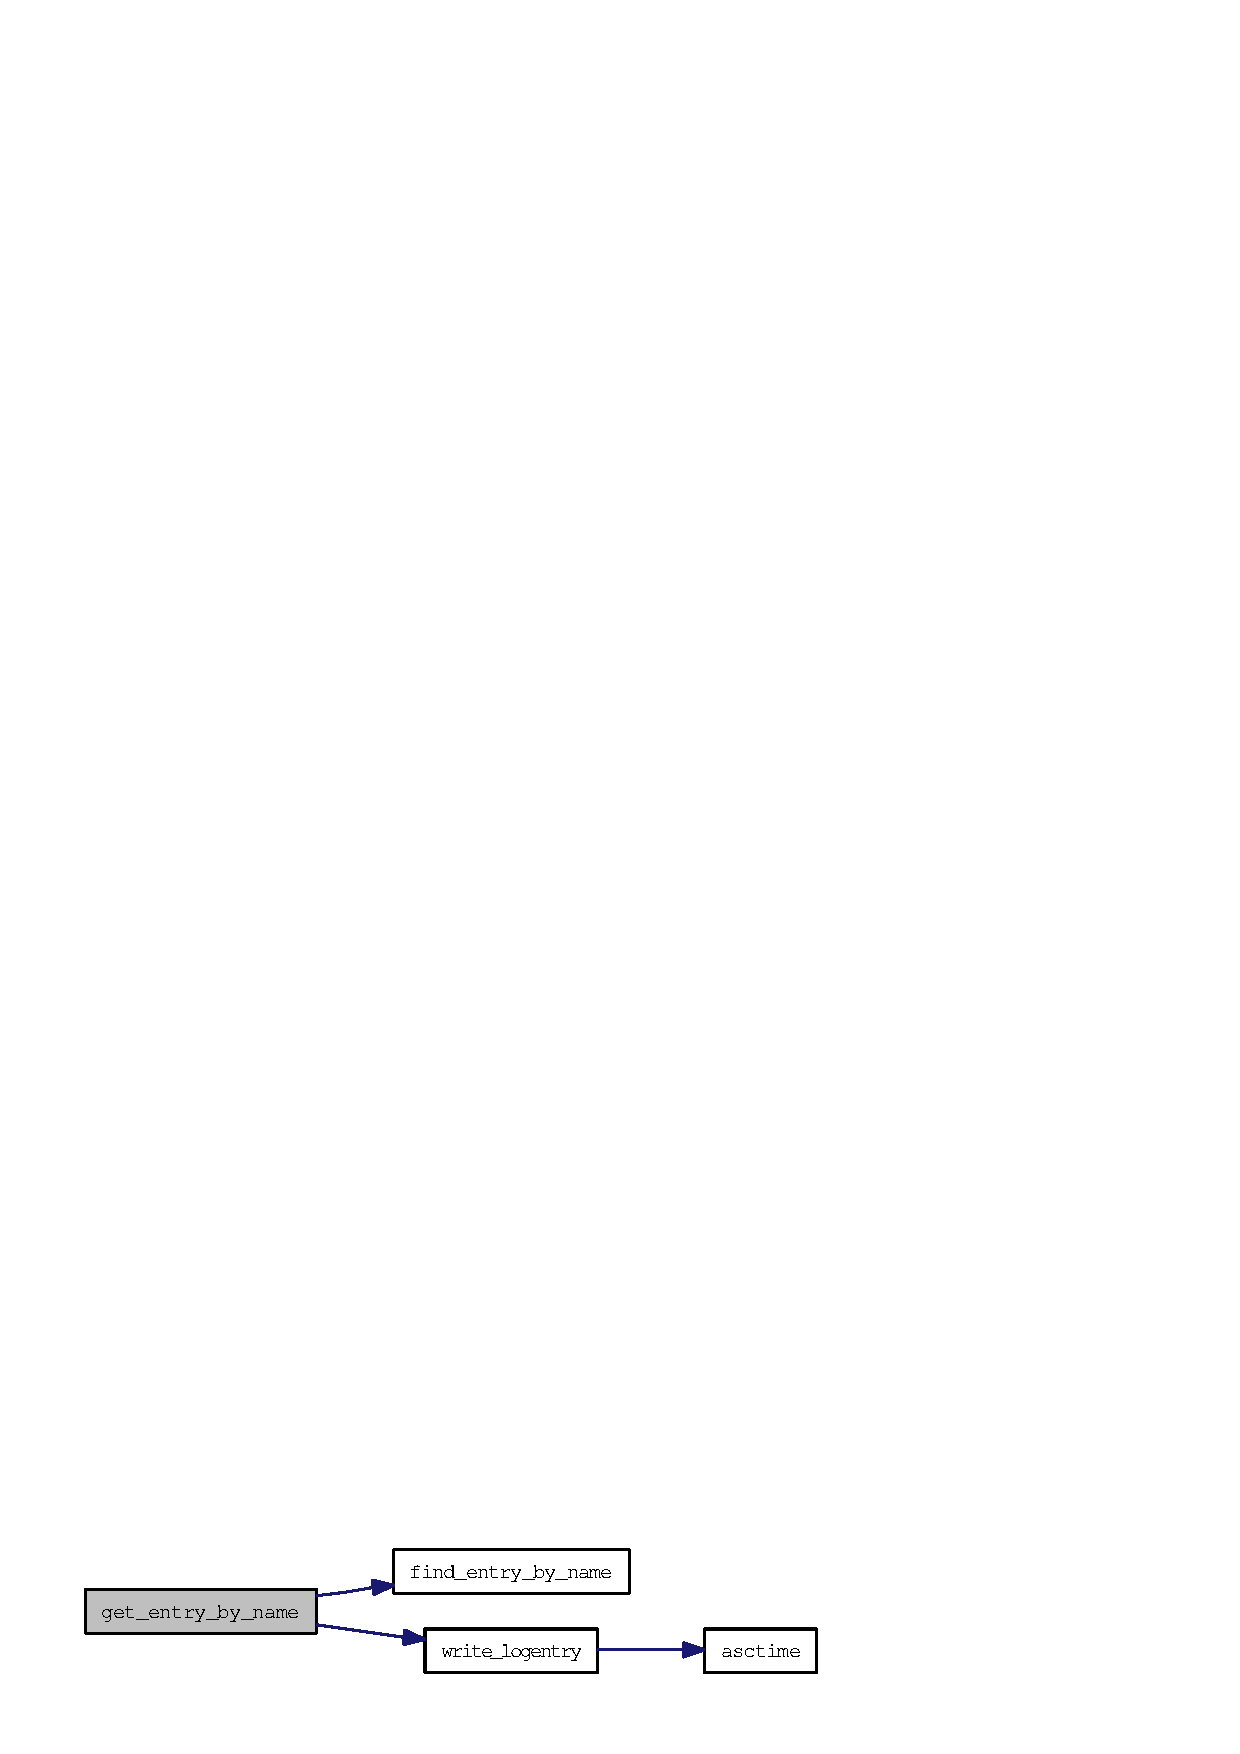
\includegraphics[width=139pt]{pf__search_8h_3947a1543660e9f6e666242efee44f89_cgraph}
\end{center}
\end{figure}
\hypertarget{pf__search_8h_678d356be18c20e298d74a62bc6e8782}{
\index{pf\_\-search.h@{pf\_\-search.h}!get\_\-entry\_\-by\_\-number@{get\_\-entry\_\-by\_\-number}}
\index{get\_\-entry\_\-by\_\-number@{get\_\-entry\_\-by\_\-number}!pf_search.h@{pf\_\-search.h}}
\subsubsection{\setlength{\rightskip}{0pt plus 5cm}struct {\bf Entry}$\ast$ get\_\-entry\_\-by\_\-number (int {\em country\_\-code}, int {\em area\_\-code}, unsigned long long {\em number}, int {\em listflag})\hspace{0.3cm}{\tt  \mbox{[}read\mbox{]}}}}
\label{pf__search_8h_678d356be18c20e298d74a62bc6e8782}


Search a entries by number (country code + area code + number).

\begin{Desc}
\item[Parameters:]
\begin{description}
\item[{\em country\_\-code}]The country code (for example 39 for Italy, 43 for Austria, and so one) \item[{\em area\_\-code}]The area code which indicates your mobile operator. \item[{\em number}]The telephone number of the person (without country and area code. \item[{\em listflag}]A flag, which indicates if you would use the blacklist (BLACKLIST\_\-FLAG) or the whitelist (WHITELIST\_\-FLAG).\par
\end{description}
\end{Desc}
\begin{Desc}
\item[Returns:]\hyperlink{structentry}{entry} Returns the entries which are found in a linked list. \end{Desc}


Definition at line 158 of file pf\_\-search.c.

References ASCII\_\-PERCENT\_\-CHAR, DB\_\-FILE, ERR\_\-LOG, find\_\-entry(), insert\_\-into\_\-list(), MAX\_\-LINE\_\-LENGTH, STMT\_\-SIZE, TB\_\-AREACODE, TB\_\-COUNTRYCODE, TB\_\-NAME, TB\_\-NUMBER, TB\_\-PRIORITY, TB\_\-REASON, and WHITELIST\_\-FLAG.

Here is the call graph for this function:\nopagebreak
\begin{figure}[H]
\begin{center}
\leavevmode
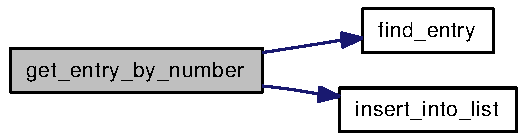
\includegraphics[width=144pt]{pf__search_8h_678d356be18c20e298d74a62bc6e8782_cgraph}
\end{center}
\end{figure}
\hypertarget{pf__search_8h_b4e0af5dc1b0cf0bdd5812c973dcd353}{
\index{pf\_\-search.h@{pf\_\-search.h}!get\_\-entry\_\-by\_\-reason@{get\_\-entry\_\-by\_\-reason}}
\index{get\_\-entry\_\-by\_\-reason@{get\_\-entry\_\-by\_\-reason}!pf_search.h@{pf\_\-search.h}}
\subsubsection{\setlength{\rightskip}{0pt plus 5cm}struct {\bf Entry}$\ast$ get\_\-entry\_\-by\_\-reason (char $\ast$ {\em reason}, int {\em listflag})\hspace{0.3cm}{\tt  \mbox{[}read\mbox{]}}}}
\label{pf__search_8h_b4e0af5dc1b0cf0bdd5812c973dcd353}


Search a entries by reason.

\begin{Desc}
\item[Parameters:]
\begin{description}
\item[{\em reason}]The reason why a person is blocked/accpeted. \item[{\em listflag}]A flag, which indicates if you would use the blacklist (BLACKLIST\_\-FLAG) or the whitelist (WHITELIST\_\-FLAG).\par
\end{description}
\end{Desc}
\begin{Desc}
\item[Returns:]\hyperlink{structentry}{entry} Returns the entries which are found in a linked list. \end{Desc}


Definition at line 206 of file pf\_\-search.c.

References ASCII\_\-PERCENT\_\-CHAR, DB\_\-FILE, ERR\_\-LOG, find\_\-entry(), insert\_\-into\_\-list(), MAX\_\-LINE\_\-LENGTH, STMT\_\-SIZE, TB\_\-AREACODE, TB\_\-COUNTRYCODE, TB\_\-NAME, TB\_\-NUMBER, TB\_\-PRIORITY, TB\_\-REASON, and WHITELIST\_\-FLAG.

Here is the call graph for this function:\nopagebreak
\begin{figure}[H]
\begin{center}
\leavevmode
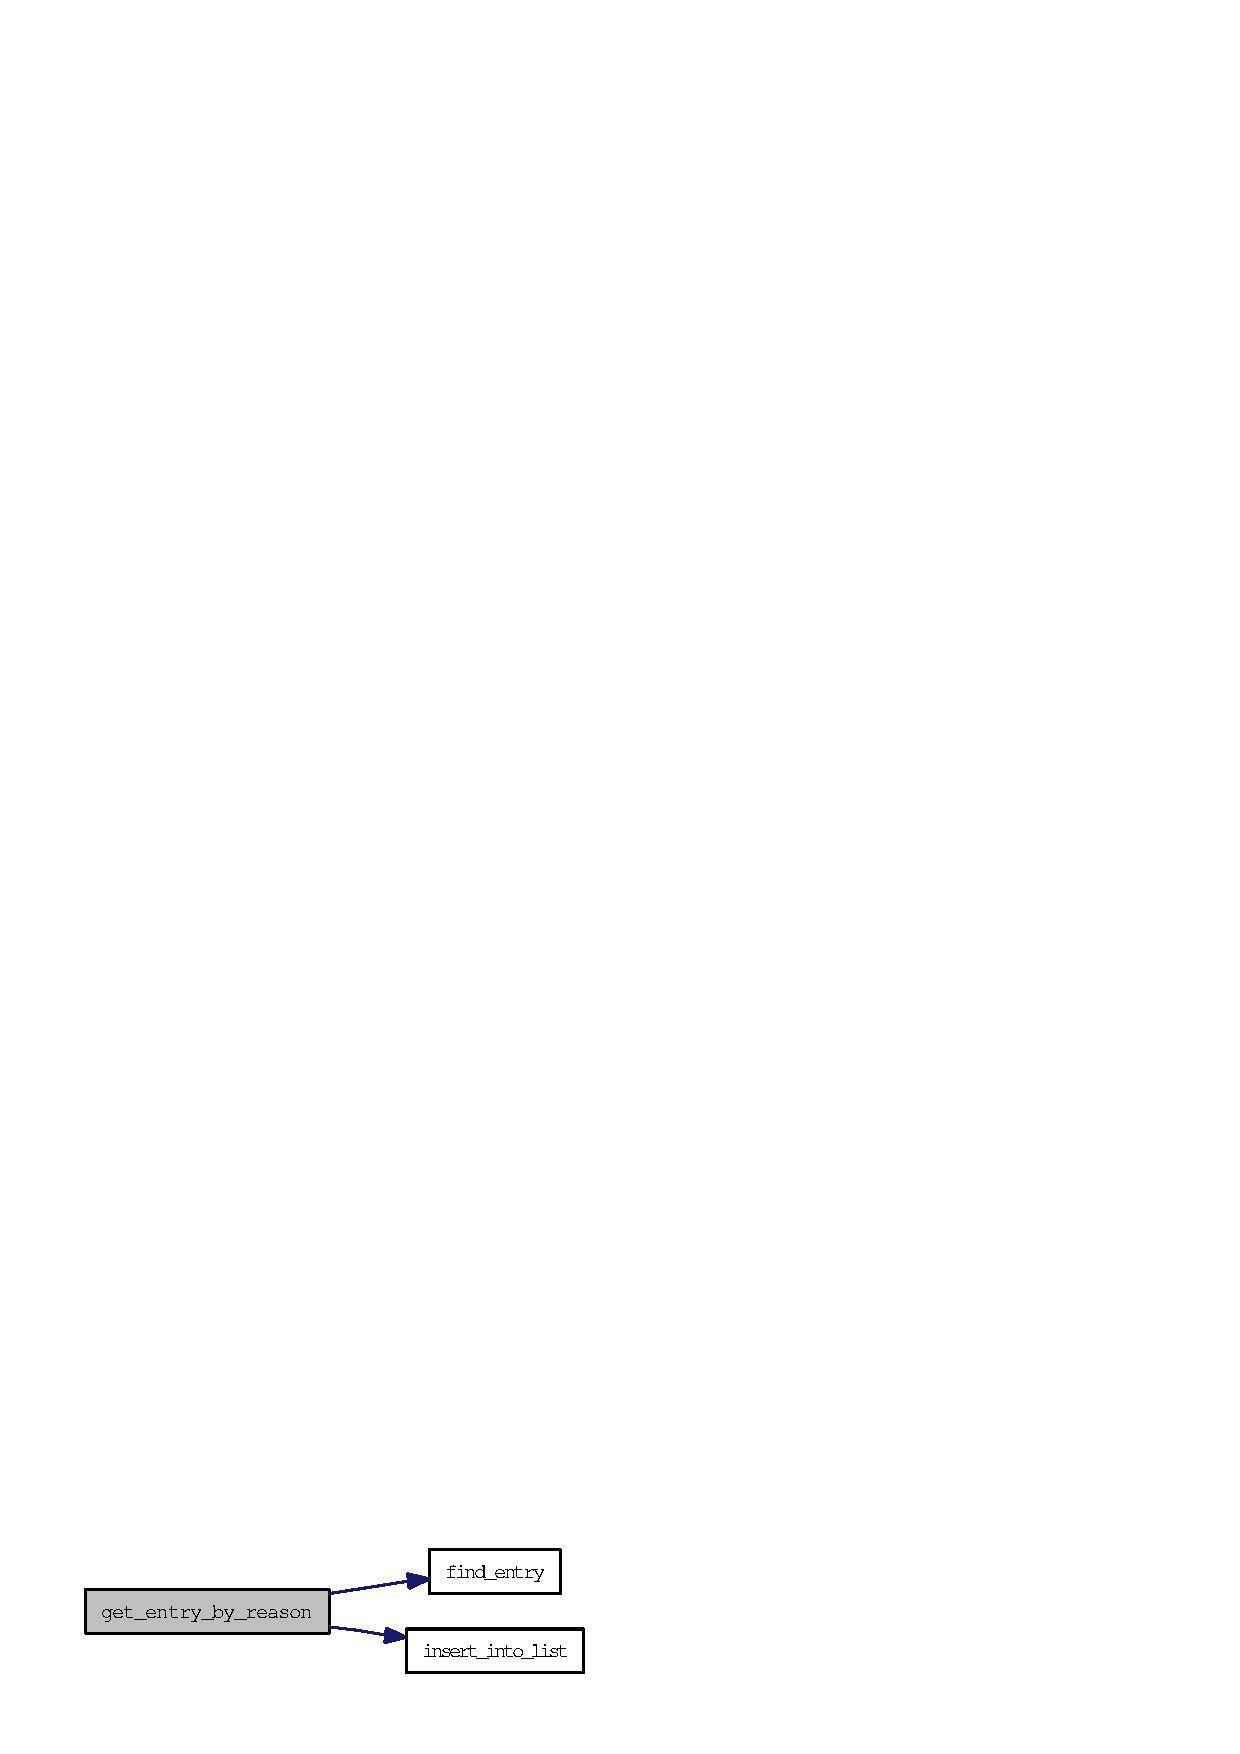
\includegraphics[width=142pt]{pf__search_8h_b4e0af5dc1b0cf0bdd5812c973dcd353_cgraph}
\end{center}
\end{figure}
